\documentclass[10pt,journal,compsoc]{IEEEtran}
\usepackage[T1]{fontenc}
\usepackage{cite}
\usepackage{amsmath,amssymb,amsfonts}
\usepackage{graphicx}
\usepackage{booktabs,tabularx,array}
\usepackage{xcolor}
\usepackage{tikz}
\usetikzlibrary{arrows.meta,positioning,fit}
\usepackage[hidelinks]{hyperref}
\usepackage{xurl}
\usepackage{subcaption}
\graphicspath{{figures/}}

\newcolumntype{Y}{>{\raggedright\arraybackslash}X}
\newcommand{\code}[1]{\texttt{\detokenize{#1}}}
\newcommand{\ind}{\mathbf{1}}
\newcommand{\reach}{\mathcal{D}}
\newcommand{\unknown}{\bot}
\definecolor{auditblue}{RGB}{26,67,107}
\definecolor{auditgold}{RGB}{168,102,24}
\interdisplaylinepenalty=2500
\newtheorem{proposition}{Proposition}
\newtheorem{theorem}{Theorem}

\newcommand{\PaperTitle}{Maintainer Prioritization in Registry-Scale Supply Chains: Multi-Objective Trade-offs, Representation Sensitivity, and Authority-Aware Hardening}

% Generated by scripts/render_research_figures.py from structural_interventions/results.json.
\newcommand{\StudyPackages}{25,228}
\newcommand{\StudyMaintainers}{12,217}
\newcommand{\StudyWorkflowPackages}{15,233}
\newcommand{\StudyWorkflowRepos}{7,171}
\newcommand{\GreedyCovered}{5,538}
\newcommand{\GreedyCoveragePercent}{77.2}
\newcommand{\GreedyExposurePercent}{11.48}
\newcommand{\UnionCovered}{4,407}
\newcommand{\UnionExposurePercent}{33.79}
\newcommand{\GreedyExcluded}{800}
\newcommand{\VersionPairsDecreasePercent}{42.44}
\newcommand{\ChangedRoots}{8,587}

% Generated rows: method, C count, C percent, H percent, P count; budget 100.
% Random row is the mean of 200 trials; figure random curve uses exact analytic expectation.
\newcommand{\ResearchMethodRows}{%
Portfolio & 4,579 & 63.9 & 7.96 & 577 \\%
Summed reach & 4,835 & 67.4 & 21.98 & 704 \\%
Maximum reach & 4,268 & 59.5 & 33.59 & 533 \\%
Exact union & 4,407 & 61.5 & 33.79 & 534 \\%
Greedy coverage & 5,538 & 77.2 & 11.48 & 800 \\%
Random (mean) & 1,680.6 & 23.4 & 0.80 & 12.8 \\%
}


\begin{document}

\title{\PaperTitle}

\author{Ashikul~Islam,~\IEEEmembership{Graduate Student Member,~IEEE,}
        and~Shahriar~Hasan,~\IEEEmembership{Member,~IEEE}%
\IEEEcompsocitemizethanks{
\IEEEcompsocthanksitem A. Islam and S. Hasan are with the Department of Computer Science and Engineering, Hajee Mohammad Danesh Science and Technology University (HSTU), Dinajpur 5200, Bangladesh.\protect\\
E-mails: ashik@hstu.ac.bd, shahriar@hstu.ac.bd.
}%
\thanks{Manuscript submitted to IEEE Transactions on Software Engineering (TSE), October 2026.}}

\markboth{IEEE Transactions on Software Engineering,~Vol.~XX, No.~Y, October~2026}%
{Islam and Hasan: Maintainer Prioritization in Registry-Scale Supply Chains}

\IEEEtitleabstractindextext{%
\begin{abstract}
Selecting maintainer accounts for review raises three different questions: how many repositories are reached, how much account-origin exposure is represented, and whether every observed source of a repository is selected. We compare these objectives in a retained npm graph of 25,228 identifiers, including 2,745 bundled contexts, and 12,217 maintainer usernames. At budget 100, greedy coverage reaches 5,538 of 7,171 workflow-associated repositories, whereas exact-union ranking reaches 4,407. Under a uniform single-account-origin scenario with perfect selected-source hardening, their exposure reductions are 11.48\% and 33.79\%, respectively. A heuristic aimed at all-source exclusion counts 1,022 repositories, compared with greedy's 800. Seven scalarization settings show intermediate coverage--exposure tradeoffs; assumed heterogeneous weights change which accounts are favored. Preserving exact version continuity reduces account--repository pairs by 42.44\%, although both representations remain observed unions. A separate bounded historical metadata reconstruction resolves 1,841 of 1,848 recorded edges; it does not recover historical installations or establish publishing authority. These results support explicit objective and observation choices in structural prioritization, without estimating compromise probabilities or deployed-control effects.
\end{abstract}

\begin{IEEEkeywords}
Software supply chain security, npm ecosystem, maintainer prioritization, multi-objective optimization, submodularity, dependency graphs, release authority.
\end{IEEEkeywords}}

\maketitle
\IEEEdisplaynontitleabstractindextext
\IEEEpeerreviewmaketitle

\section{Introduction}
\IEEEPARstart{N}{pm} dependency and maintainer relations can concentrate downstream reach in a small set of accounts. Earlier ecosystem studies measured this concentration and proposed maintainer vetting and metadata-based review signals~\cite{zimmermann2019,zahan2022}. A defensive program still needs to decide what a limited account-review budget should accomplish. Distinct repository coverage, exposure across account-origin scenarios, and selection of every observed source are different quantities.

Consider two accounts whose package portfolios reach many of the same repositories. Selecting the first may leave little additional coverage for the second. Nevertheless, an unselected second account remains a possible origin in the structural model. A repository can therefore be covered while retaining most of its observed sources. This is an objective distinction, not evidence that either account was compromised or that review would prevent compromise.

Our study extends established reach and greedy-coverage baselines~\cite{zimmermann2019,nemhauser1978} by measuring three objectives on the same observed incidence relation. We evaluate five deterministic selection rules, 200 random orders and six budgets. We then examine exact-version continuity, endpoint deduplication, observation exclusions, and hybrid and exclusion-oriented selections. The graph contains 25,228 identifiers and 12,217 usernames; workflow-positive package observations map to 7,171 repository keys. These are the units in a seeded expansion, rather than a representative sample of npm installations.

October 2026 reports illustrate boundaries that this graph cannot resolve. LiteLLM described master-key exposure, CI secret theft and misuse of developer tokens~\cite{litellm2026}, with published artifacts differing from a source tag~\cite{litellmincident2026}. The incident concerns PyPI/container releases, not an npm validation case. Pillar's OpenCode disclosure concerned a legacy npm dependency on Windows/WSL~\cite{opencode2026}. Railway described possible environment-variable exposure and a deployment pause~\cite{railway2026,railwaydisclosure2026}. SlugFest concerned publishing trust bindings~\cite{npmtrustedpub2026,npmexpiry2026}; the Node.js Brotli disclosure concerns a runtime outside the package graph~\cite{nodejsbrotli2026}. We retain these as contextual boundaries, without deriving intervention efficacy from them.

We ask five questions:
\begin{itemize}
\item \textbf{RQ1:} How do distinct coverage and additive scenario exposure differ at equal account budgets?
\item \textbf{RQ2:} How many covered repositories retain unselected sources, and what does an exclusion-oriented heuristic change?
\item \textbf{RQ3:} How do graph representation and selection/evaluation combinations affect the measured results?
\item \textbf{RQ4:} What tradeoffs arise under scalarized objectives and assumed heterogeneous weights?
\item \textbf{RQ5:} Which historical metadata can be reconstructed, and which evidence remains missing for authority-aware outcome evaluation?
\end{itemize}

The contribution is a measured comparison of established structural objectives, their representation and observation sensitivities, and the limits of the retained metadata. The scalarized objective has a standard submodular guarantee; our seven greedy settings do not certify a global Pareto frontier. The direct exclusion rule is a heuristic. The historical companion and frozen prospective acquisition pilot supply feasibility evidence, without a fitted forecasting model or deployed-control evaluation.

\section{Related Work}
\label{sec:related_work}

Our research intersects five major areas of empirical software engineering and software supply-chain security: structural ecosystem measurement, malicious package detection, continuous-integration workflow analysis, registry governance and provenance, and temporal dependency reconstruction.

\subsection{Ecosystem Structure and Centrality-Based Prioritization}
Pioneering empirical studies established that open-source package registries exhibit extreme structural asymmetry and small-world properties. Zimmermann et al.~\cite{zimmermann2019} analyzed npm's dependency topology, revealing that a tiny core of central packages and maintainers transitively affects a vast majority of the ecosystem. Zahan et al.~\cite{zahan2022} study metadata weak-link signals, while Liu et al.~\cite{liu2022} examine dependency-tree vulnerability propagation.

Zimmermann et al.~\cite{zimmermann2019} already studied maintainer-union reach, greedy coverage, and vetting. Wang~\cite{wang2026} evaluates package-node protection in cascade simulations. Our contribution is an empirical comparison of coverage, account-origin exposure, and all-source exclusion at workflow-associated repository endpoints. We evaluate established baselines and a stated heuristic, without claiming a new coverage algorithm or demonstrating that PageRank fails in an experiment where it was not evaluated.

\subsection{Malicious Package Benchmarks and Detection Limits}
A parallel line of security research focuses on detecting malicious packages published via typosquatting, dependency confusion, and account takeovers~\cite{ohm2020,sejfia2022}. Benchmark evaluations, such as Guo et al.'s extensive study of npm malware detectors~\cite{guo2026}, show that static analysis tools face severe limitations due to obfuscation, dynamic runtime execution, and environment-keyed payloads. 

Because reactive post-publication malware detection suffers from non-trivial evasion rates, proactive hardening of legitimate, high-leverage maintainer accounts is a complementary research direction~\cite{schorlemmer2024,okafor2025}. Our work complements malware detection by optimizing how defenders allocate proactive security interventions before credentials or tokens are compromised.

\subsection{Continuous-Integration Workflows and Reachability Limits}
Software supply-chain risks manifest concretely in downstream CI/CD pipelines. Koishybayev et al.~\cite{koishybayev2022} and Muralee et al.~\cite{muralee2023} demonstrated that GitHub Actions workflows frequently execute third-party build scripts with access to repository secrets, cloud deployment credentials, and package publish tokens. Recent incidents motivate artifact-level checks: Railway's preliminary report describes potential secret exposure affecting at most 1.85\% of workspaces, approximately 100,000, and notes that builds had resumed~\cite{railway2026}. LiteLLM reported a release workflow redirected to attacker-controlled source, with separate approval and log-deletion credentials~\cite{litellm2026}. These are contextual examples rather than observations in our npm graph.

Crucially, recent empirical studies have emphasized that package-level dependency relationships do not equal actual code execution. Weeraddana, Alfadel, and McIntosh~\cite{weeraddana2024} studied CI time spent updating unused npm dependencies. Shen et al.~\cite{gao2025emse} reported that 99\% of client vulnerabilities in their studied corpus arose from dependencies and 81.26\% of package-level findings were false positives under finer analysis. These corpus-specific results do not establish registry-wide false-positive rates. Jayasuriya et al.~\cite{jayasuriya2024} observed similar granularity effects when analyzing syntactic breaking changes across versions. In our work, we address this fundamental reachability gap by evaluating both coarse package-name projections and version-continuous graphs, treating topological reach as a conditional review surface rather than installed-code evidence.

\subsection{Registry Governance, Cryptographic Provenance, and Signing}
In response to account compromises, registries and standards bodies have introduced cryptographic signing and provenance attestations. Schorlemmer et al.~\cite{schorlemmer2024} audited signing across Maven, PyPI, Docker Hub, and Hugging Face, finding that adoption remains minimal and unevenly distributed. Kalu et al.~\cite{okafor2025} interviewed industry practitioners, revealing significant operational friction in managing cryptographic keys and configuring automated pipeline attestations. Bloom Security's SlugFest disclosure concerns mutable repository-name bindings before a first trusted publish, rather than a break of OIDC cryptography~\cite{npmtrustedpub2026}. GitHub announced expiry of unvalidated bindings on October 2~\cite{npmexpiry2026}; reported exposure is not evidence that all affected packages were maliciously published. Pillar's October 19 OpenCode report describes a September 28 dependency fix without a CVE~\cite{opencode2026}, illustrating a coverage gap for CVE-indexed detection.

Simultaneously, He, Vasilescu, and K{\"a}stner~\cite{he2025} demonstrated that local dependency version pinning is insufficient to protect clients against upstream attacks, as adversaries exploit unpinned sub-dependencies and registry-level re-resolutions. These findings motivate examining account controls alongside version and artifact evidence; they do not establish control efficacy in our graph.

\subsection{Temporal Reconstruction and Empirical Standards}
A critical methodological vulnerability in supply-chain studies is future-leakage bias---evaluating historical attacks using contemporary registry graphs. Pinckney et al.~\cite{pinckney2023} introduced \texttt{npm-follower} to mirror registry event streams, while Rahman et al.~\cite{rahman2026} released \texttt{CHRONO-RESOLUTION} to reconstruct exact dependency trees at release points. Shafin and Ahmed~\cite{shafin2026} highlighted the necessity of time-indexed forecasting.

Our reporting is informed by the ACM SIGSOFT Empirical Standards~\cite{ralph2020}. By avoiding pseudo-replication---specifically rejecting the treat\-ment of fixed-graph nested budgets or repeated random orders as independent sampling units---our study provides reproducible descriptive comparisons and exploratory scalarization results.

\begin{table*}[t]
\centering
\small
\caption{Selected literature and the scope of our empirical investigation relative to major related literature.}
\label{tab:lit_positioning}
\begin{tabularx}{\textwidth}{lYYYY}
\toprule
\textbf{Research Dimension} & \textbf{Structural Topology \& Centrality} & \textbf{Malicious Package Detectors} & \textbf{CI/CD \& Function Call-Graphs} & \textbf{This Study (Q1 Journal Expansion)} \\
\midrule
\textbf{Focus Literature} & Zimmermann~\cite{zimmermann2019}, Zahan~\cite{zahan2022}, Wang~\cite{wang2026} & Ohm~\cite{ohm2020}, Sejfia~\cite{sejfia2022}, Guo~\cite{guo2026} & Koishybayev~\cite{koishybayev2022}, Weeraddana~\cite{weeraddana2024}, Shen~\cite{gao2025emse} & Structural objectives ($C, H, P, J_\alpha$), version continuity, field availability \\
\midrule
\textbf{Prioritization Metric} & Dependency and maintainer reach; coverage; metadata signals & Reactive post-event incident signatures & Taint analysis on workflows, call-graph reachability & Submodular coverage, modular exposure reduction, supermodular all-source exclusion \\
\midrule
\textbf{Graph Representation} & Dependency graphs and resolved trees & Isolated package tarballs & Dynamic execution traces, static ASTs & Dual evaluation: Package-projected vs. Version-continuous closures (42.4\% pair diff) \\
\midrule
\textbf{Maintainer Risk Prior} & Uniform equal weight & Unweighted & Unweighted & Heterogeneous weights: Solo bottlenecks ($H_{\text{sole}}$), log-portfolio ($H_{\text{log}}$), package-level sole reach ($H_{\text{pkg-sole}}$) \\
\midrule
\textbf{Temporal Grounding} & Static single snapshot & Retrospective positive-only datasets & Static GitHub Actions scripts & 45 root records (44 distinct tuples), 1,848 bounded edge attempts ($t_{\text{cutoff}} < t_{\text{incident}}$), 90-day prospective cohort \\
\bottomrule
\end{tabularx}
\end{table*}

\section{Data Corpus and Graph Construction}
\label{sec:data_construction}
\subsection{Collection and Units}
The collector seeds a high-impact npm list, expands dependencies through deps.dev~\cite{depsdevapi}, requests registry metadata, and checks linked GitHub repositories for a \code{.github/workflows} directory at HEAD. Queue dates span June 13--16, 2026, but individual fields lack a common acquisition cutoff. The retained archive analyzed on October 20 contains 25,228 graph identifiers, 22,340 version-metadata rows, 12,217 maintainer usernames, and 79,405 package--maintainer relations. Maintainer membership is not a historical publisher log.

Among these identifiers, 2,745 encode bundled contexts rather than independently registered packages. The 121,885 retained version-edge rows project to 88,113 distinct name adjacencies. Stored \code{DIRECT}/\code{INDIRECT} labels describe a target node relative to an extraction root; their 48,705/73,180 row counts do not partition global direct and transitive edges~\cite{depsdevapi}. We reverse every explicit declaring-to-dependency adjacency to measure downstream reach.

\begin{figure*}[t]
\centering
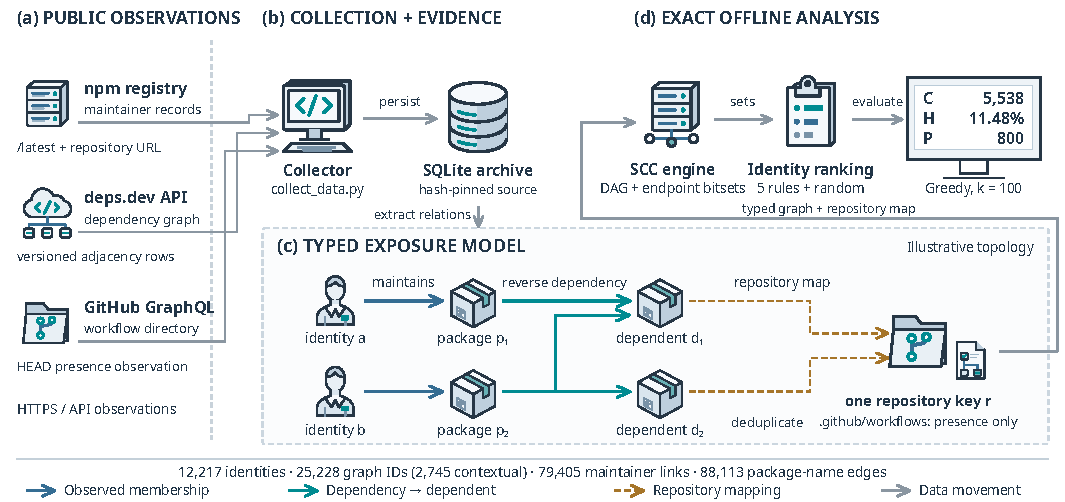
\includegraphics[width=0.96\textwidth]{study_system.pdf}
\caption{Implemented measurement architecture. Icons denote logical roles and topology is illustrative. Counts and displayed greedy outcomes are empirical; workflow presence does not establish execution.}
\label{fig:q1_observation_workflow}
\end{figure*}

The 15,233 workflow-positive package names map to 7,171 normalized repository keys. Owner/name pairs are case-folded and trailing transport \code{.git} is removed. This is lexical deduplication, without redirect or commit verification. There are 3,081 identifiers without maintainer mappings and 3,772 without completed workflow flags. Zero flags conflate directory absence with repository unavailability. Workflow endpoints require a positive observation; missing and zero flags are not evidence of safety. Coverage uses all 7,171 repository endpoints. Only 7,158 have an observed source identity; the other 13 are excluded from source-exclusion counts.

\begin{figure*}[t]
\centering
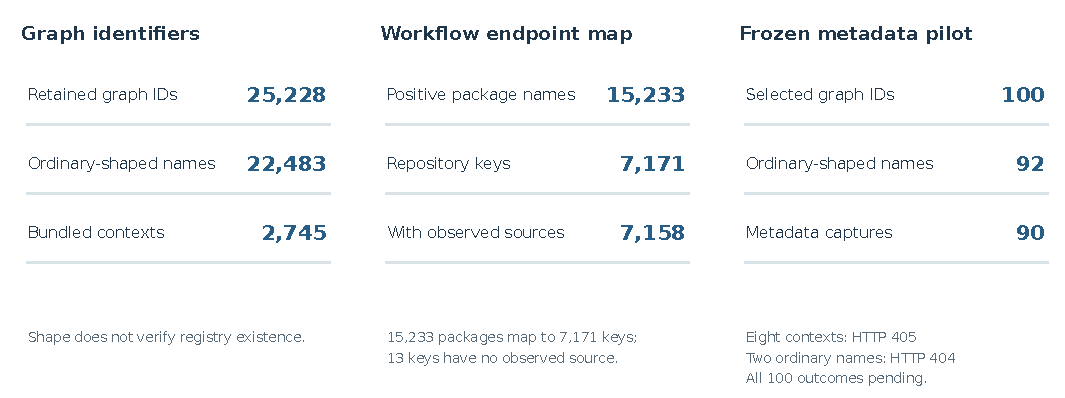
\includegraphics[width=0.94\textwidth]{observation_scope.pdf}
\caption{Observation units and prospective acquisition. Panels describe separate populations; their missingness counts must not be added across panels. Context identifiers are retained graph units, not separate registry packages. The prospective selection was frozen before requests; all 100 outcomes remain pending.}
\label{fig:q1_observation_scope}
\end{figure*}

Figure~\ref{fig:q1_observation_scope} separates graph units, observed workflow endpoints, and the prospective selection frame. This distinction matters because directory observation and metadata acquisition do not validate a historical installation or a future outcome.

\subsection{Name Projection and Exact-Version Continuity}
The name graph merges retained versions sharing an identifier. The sensitivity graph retains 40,806 exact (package, version) nodes and joins paths only at matching version keys. A maintained package seeds every retained version; without a version node, it contributes only its eligible seed endpoint. Both representations use the same package-level workflow flags. Neither reproduces npm installation or historical lockfile behavior: contexts and acquisition times remain mixed.

\begin{figure}[t]
\centering
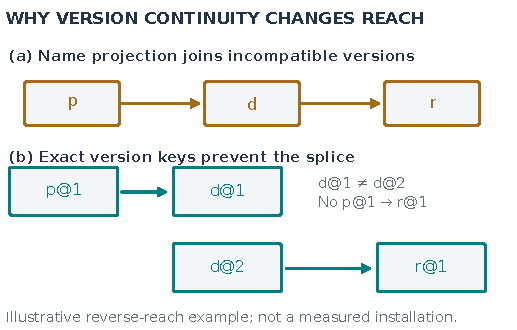
\includegraphics[width=\columnwidth]{graph_semantics.pdf}
\caption{Illustrative version splicing. Collapsing intermediate versions creates a name-level path without an exact-version counterpart. Reverse-reach arrows do not describe a measured installation.}
\label{fig:q1_version_semantics}
\end{figure}

\subsection{Cycles, Mapping Disagreements and Contexts}
The name graph has 82 nontrivial strongly connected components (SCCs) containing 403 nodes; the exact-version union has 68 containing 304 nodes. The largest component has 61 nodes in each. SCC condensation preserves reach and permits exact bitset propagation over a directed acyclic graph; the implementation uses arbitrary-precision Python integers, not fixed 64-bit sets. This is a computation technique, not an intervention that removes cycles.

The URL audit finds 658 identifier-level parser disagreements. Excluding 60 inconsistent positive observations reduces the workflow repository universe to 7,147; greedy at budget 100 gives $C=5{,}524$ and $P=799$. We discard ambiguous flags rather than transferring them to a corrected URL without reacquisition. Removing bundled-context nodes preserves all 462,170 primary account--repository incidences for fixed selections, although workflow-package incidence changes. That invariance does not apply automatically to every endpoint definition or individual-package ranking.

\section{Objectives and Optimization Framework}
\label{sec:objectives}

Maintainer prioritization in package registries represents a multi-objective decision problem under a fixed hardening budget $k = |S|$. Let $M$ denote the universe of maintainers ($|M| = 12,217$) and $R_{\text{wf}}$ denote the universe of downstream workflow repositories ($|R_{\text{wf}}| = 7,171$). For each maintainer $m \in M$, let $E_m \subseteq R_{\text{wf}}$ denote the set of repositories reachable from packages authored by $m$, and let $\text{Sources}(r) = \{m \in M : r \in E_m\}$ denote the upstream maintainer set of repository $r$.

\subsection{Formal Objective Definitions}
We formalize three fundamental defensive quantities:

\subsubsection{Submodular Distinct Coverage ($C(S)$)}
Defenders seeking broad ecosystem review prioritize distinct downstream client repositories:
\begin{equation}
C(S) = \left| \bigcup_{m \in S} E_m \right|
\end{equation}
\textbf{Property:} $C(S)$ is normalized, monotone non-decreasing, and strictly submodular. For any subsets $A \subseteq B \subseteq M$ and element $m \notin B$:
\begin{equation}
C(A \cup \{m\}) - C(A) \ge C(B \cup \{m\}) - C(B)
\end{equation}
The classic result of Nemhauser, Wolsey, and Fisher~\cite{nemhauser1978} establishes that the greedy algorithm selecting $m^* = \arg\max_{m \notin S} |E_m \setminus \bigcup_{u \in S} E_u|$ achieves a $(1 - 1/e) \approx 63.2\%$ approximation of the optimal coverage.

\subsubsection{Modular Scenario Exposure Reduction ($H(S)$)}
In threat models where each maintainer account represents an independent compromise event with prior probability weight $w_m$, defenders seek to eliminate the greatest expected downstream exposure mass:
\begin{equation}
H(S) = \frac{\sum_{m \in S} w_m |E_m|}{\sum_{v \in M} w_v |E_v|}
\end{equation}
\textbf{Property:} $H(S)$ is normalized, monotone, and strictly \textit{modular} (additive linear). For any disjoint sets $A, B \subseteq M$, $H(A \cup B) = H(A) + H(B)$. Consequently, exact-union ranking (sorting maintainers in descending order of weighted reach $w_m |E_m|$) is mathematically guaranteed to achieve the exact global optimum for $H(S)$ at any budget $k$.

\subsubsection{Supermodular All-Source Exclusion ($P(S)$)}
A client repository $r$ is fully insulated against single-account compromise if and only if \textit{every} maintainer in its upstream dependency tree has adopted hardening controls:
\begin{equation}
P(S) = \sum_{r \in R_{\text{wf}}} \mathbb{I}[\text{Sources}(r) \subseteq S]
\end{equation}
\textbf{Property:} $P(S)$ is strictly \textit{supermodular}. Selecting maintainer $m$ contributes zero gain to $r$ until the final remaining unhardened maintainer of $r$ is selected, producing sharp threshold transitions:
\begin{equation}
P(A \cup \{m\}) - P(A) \le P(B \cup \{m\}) - P(B) \quad \text{for } A \subseteq B
\end{equation}

\subsection{Proposition 1: Monotone Submodularity of Hybrid Scalarization $J_\alpha(S)$}
Because single-objective optimization induces severe polarization between $C(S)$ and $H(S)$, we formulate a hybrid scalarization function:
\begin{equation}
J_\alpha(S) = \alpha \cdot \frac{C(S)}{|R_{\text{wf}}|} + (1 - \alpha) \cdot H(S)
\end{equation}
where $\alpha \in [0, 1]$ parameterizes defensive posture between broad coverage ($\alpha = 1$) and scenario exposure reduction ($\alpha = 0$).

\begin{proposition}
For any $\alpha \in [0, 1]$, the marginal gain function $\Delta J_\alpha(m \mid S) = J_\alpha(S \cup \{m\}) - J_\alpha(S)$ is monotone non-decreasing and submodular.
\end{proposition}
\begin{IEEEproof}
Let $A \subseteq B \subseteq M$ and $m \notin B$. The marginal gain is:
\begin{equation}
\Delta J_\alpha(m \mid S) = \alpha \frac{|E_m \setminus \bigcup_{u \in S} E_u|}{|R_{\text{wf}}|} + (1 - \alpha) \frac{w_m |E_m|}{\sum_{v \in M} w_v |E_v|}
\end{equation}
The second term is constant with respect to $S$ (modular), so its marginal difference across $A$ and $B$ is exactly zero. The first term satisfies submodularity by set-theoretic inclusion:
\begin{equation}
|E_m \setminus \bigcup_{u \in A} E_u| \ge |E_m \setminus \bigcup_{u \in B} E_u|
\end{equation}
Because the sum of a submodular set function and a modular set function is submodular, $J_\alpha(S)$ is submodular for all $\alpha \in [0, 1]$. By the Nemhauser bound~\cite{nemhauser1978}, accelerated lazy greedy optimization achieves at least a $(1 - 1/e)$ approximation of the optimum scalarized objective.
\end{IEEEproof}

\subsection{Supermodular Minimum-Remaining-Source Heuristic for $P(S)$}
Because $P(S)$ is supermodular, greedy coverage and exact union achieve all-source exclusion purely as an unoptimized side-effect. To directly optimize $P(S)$, we design an adaptive minimum-remaining-source heuristic. At each step, let $\text{rem}(r) = \text{Sources}(r) \setminus S$. The heuristic scores unselected maintainers by:
\begin{equation}
\text{Score}(m) = \sum_{r : \text{rem}(r) = \{m\}} 1 + \sum_{r : m \in \text{rem}(r), |\text{rem}(r)| > 1} \frac{1}{|\text{rem}(r)|}
\end{equation}
breaking ties by marginal coverage $|E_m \setminus \bigcup_{u \in S} E_u|$.

\subsection{Heterogeneous Maintainer Risk Formulations}
We evaluate three structural models of non-uniform maintainer risk:
\begin{enumerate}
    \item \textbf{Single-Maintainer Bottlenecks ($w_m^{\text{sole}}$):} Packages with $|M(p)| = 1$ lack peer review. We weight maintainers by $w_m^{\text{sole}} = 1 + |\{p \in P_m : |M(p)| = 1\}|$.
    \item \textbf{Log-Portfolio Activity ($w_m^{\text{log}}$):} Token attack surface scales logarithmically with portfolio size: $w_m^{\text{log}} = 1 + \log_2(1 + |P_m|)$.
    \item \textbf{Package-Level Sole-Maintainer Reach ($H_{\text{pkg-sole}}$):} Instead of weighting all reachable repositories of maintainer $m$, we isolate repositories reachable strictly through $m$'s sole-authored packages: $E_m^{\text{sole}} = \bigcup_{p \in P_m, |M(p)|=1} \reach(p)$.
\end{enumerate}

\subsection{Analytic Expectations and Empirical Standard Errors}
Under a finite population of $|M| = 12,217$ maintainers, random selection of budget $k$ yields exact expected coverage and exposure under the hypergeometric distribution:
\begin{align}
E[H_{\text{rand}}(k)] &= \frac{k}{|M|}, \\
E[C_{\text{rand}}(k)] &= \sum_{r \in R_{\text{wf}}} \left( 1 - \frac{\binom{|M| - |\text{Sources}(r)|}{k}}{\binom{|M|}{k}} \right).
\end{align}
For $k = 100$, exact finite-population expectations are $E[C] = 1,716.8$ and $E[H] = 0.819\%$. Across 200 simulation seeds, the sample mean coverage is 1,680.6 (sample standard deviation $\text{SD}_C = 530.7$, Monte Carlo Standard Error $\text{MCSE}_C = 37.5$), and sample mean exposure reduction is $0.819\%$ ($\text{SD}_H = 0.373\text{ pp}$, $\text{MCSE}_H = 0.026\text{ pp}$). Replicated offline execution across 3 independent runs averaged $39.50\text{ s}$ wall-clock time with $1,038.43\text{ MiB}$ peak RSS.

\section{Core Tradeoffs and Representation: RQ1 and RQ2}
\label{sec:empirical_results}

We first report our empirical findings for Research Questions 1 and 2 on the retained 25,228-identifier graph, spanning multi-budget trade-offs, multi-homing mechanics, and representation fidelity.

Figure~\ref{fig:q1_source_partition} partitions covered endpoints by whether any unselected source remains.

\begin{figure}[t]
\centering
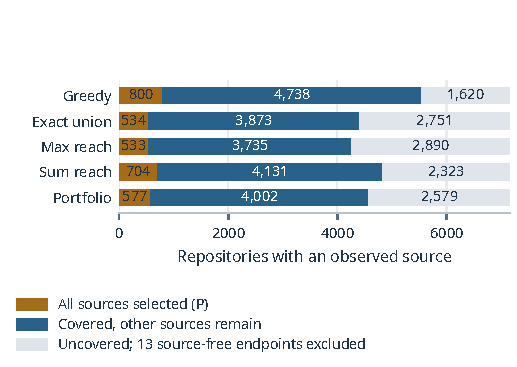
\includegraphics[width=\columnwidth]{coverage_partition.pdf}
\caption{Budget-100 repository partition. Each bar separates all-source exclusion, coverage with residual sources, and uncovered endpoints. The 13 source-free endpoints are omitted. Structural coverage and complete exclusion differ for every baseline.}
\label{fig:q1_source_partition}
\end{figure}

\subsection{RQ1: Coverage vs. Additive Exposure Trade-Off}
Figure~\ref{fig:objective_tradeoff} shows the coverage and exposure trajectories. Table~\ref{tab:multi_budget_comparison} reports empirical prioritization outcomes across maintainer budgets $|S| \in \{1, 5, 10, 25, 50, 100\}$. The top 100 maintainers represent only $0.819\%$ of the 12,217 unique maintainers in our ecosystem, yet their prioritization commands vast reach over downstream workflow repositories.

% Generated by scripts/reconcile_full_manuscript.py
\begin{table*}[t]
\centering
\footnotesize
\caption{Workflow-repository outcomes from the retained baseline experiment. Random entries are 200-order sample means and Monte Carlo standard errors, not population confidence intervals.}
\label{tab:multi_budget_comparison}
\begin{tabular}{llrrrrrr}
\toprule
Budget & Metric & Portfolio & Sum & Max & Exact union & Greedy & Random mean $\pm$ MCSE\\
\midrule
1 & C (\%) & 23.43 & 33.02 & 28.75 & 35.46 & 35.46 & 0.65 $\pm$ 0.19\\
1 & H (\%) & 0.36 & 0.51 & 0.45 & 0.55 & 0.55 & 0.01 $\pm$ 0.00\\
1 & P & 1 & 26 & 2 & 269 & 269 & 0.28 $\pm$ 0.15\\
5 & C (\%) & 46.00 & 49.25 & 42.14 & 50.96 & 54.00 & 2.61 $\pm$ 0.36\\
5 & H (\%) & 1.16 & 2.15 & 2.23 & 2.45 & 2.09 & 0.04 $\pm$ 0.01\\
5 & P & 316 & 325 & 80 & 329 & 327 & 0.69 $\pm$ 0.17\\
10 & C (\%) & 47.90 & 51.75 & 42.81 & 54.53 & 60.40 & 4.73 $\pm$ 0.46\\
10 & H (\%) & 1.59 & 2.68 & 4.06 & 4.48 & 3.79 & 0.08 $\pm$ 0.01\\
10 & P & 391 & 399 & 111 & 343 & 351 & 1.21 $\pm$ 0.19\\
25 & C (\%) & 56.71 & 60.95 & 45.29 & 59.74 & 67.69 & 10.15 $\pm$ 0.55\\
25 & H (\%) & 4.38 & 7.45 & 9.00 & 9.86 & 6.08 & 0.21 $\pm$ 0.01\\
25 & P & 430 & 480 & 116 & 427 & 514 & 2.86 $\pm$ 0.26\\
50 & C (\%) & 62.00 & 63.78 & 45.56 & 60.26 & 72.46 & 16.73 $\pm$ 0.56\\
50 & H (\%) & 6.14 & 13.72 & 17.19 & 18.09 & 8.73 & 0.43 $\pm$ 0.02\\
50 & P & 503 & 576 & 117 & 441 & 638 & 5.97 $\pm$ 0.38\\
100 & C (\%) & 63.85 & 67.42 & 59.52 & 61.46 & 77.23 & 23.44 $\pm$ 0.52\\
100 & H (\%) & 7.96 & 21.98 & 33.59 & 33.79 & 11.48 & 0.80 $\pm$ 0.03\\
100 & P & 577 & 704 & 533 & 534 & 800 & 12.78 $\pm$ 1.42\\
\bottomrule
\end{tabular}
\end{table*}



\begin{figure*}[t]
\centering
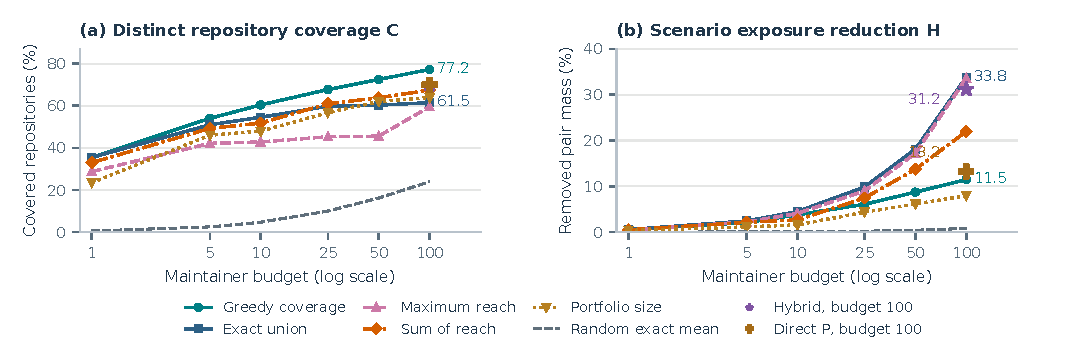
\includegraphics[width=0.92\textwidth]{objective_tradeoff.pdf}
\caption{Multi-budget trade-off trajectories across maintainer budgets $|S| \in [1, 100]$: (a) submodular coverage $C(S)$, (b) modular scenario exposure reduction $H(S)$, using five deterministic rules and the exact random expectation. Budget-100 markers show hybrid and direct-exclusion selections.}
\label{fig:objective_tradeoff}
\end{figure*}

At budget $|S|=100$, \textbf{Greedy Coverage} achieves $C(S) = 5{,}538$ repositories ($77.23\%$), establishing a descriptive lead of $+1{,}131$ repositories ($+15.77$ percentage points) over \textbf{Exact Union} ($C(S) = 4{,}407$, $61.46\%$). However, when evaluated under scenario-weighted additive exposure reduction $H(S)$, Exact Union achieves $33.79\%$, outpacing Greedy Coverage ($11.48\%$) by \textbf{$+22.30$ percentage points} ($2.94\times$ relative advantage).

Exact union's H advantage follows from its additive objective under equal costs. The experiment measures the accompanying loss in distinct coverage. Greedy offers the largest measured coverage among the compared baseline selections; it is an approximation to maximum coverage, not a proved global optimum. Portfolio size gives 63.85\% coverage and 7.96\% H at this budget, showing that portfolio count and measured downstream reach need not agree.

\subsection{Residual Sources and Single-Source Fragility}
A repository can have many source accounts even when a single account already covers it. Across the 7,158 repositories with observed sources, mean source cardinality is 64.57 and the maximum is 1,502. These are graph source identities, not measured permissions or independent compromises. Figure~\ref{fig:q1_source_distribution} shows their distribution and the remaining-source distributions after budget-100 selections.

\begin{figure*}[t]
\centering
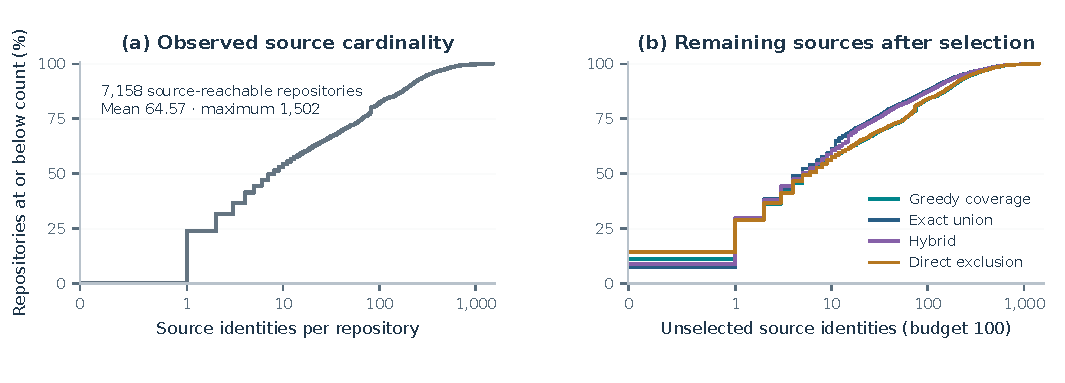
\includegraphics[width=0.94\textwidth]{source_multiplicity.pdf}
\caption{Observed source multiplicity and residual-source distributions at budget 100. All curves use the same 7,158 source-reachable repositories; 13 source-free endpoints are excluded. Zero remaining sources identify all-source exclusions. Horizontal scales are logarithmic above one. Account origins are structural scenarios, not observed compromises.}
\label{fig:q1_source_distribution}
\end{figure*}

Greedy's $P=800$ is 11.18\% of source-reachable repositories; exact union gives $P=534$. Consequently, 6,358 source-reachable repositories retain at least one unselected source after greedy selection. A four-source illustration would retain three source identities when one is selected, but that fraction is not an estimated compromise probability.

\begin{figure}[t]
\centering
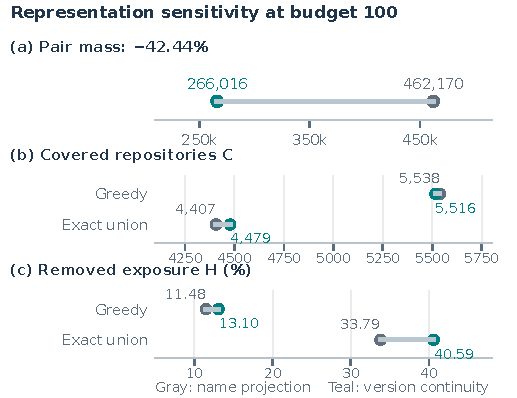
\includegraphics[width=\columnwidth]{representation_detail.pdf}
\caption{Cross-representation divergence: preserving exact-version continuity removes some paths introduced by version merging and reduces total identity-repository exposure pairs by $42.44\%$, shifting maintainer leverage. Gray denotes name projection and teal denotes version continuity.}
\label{fig:representation_detail}
\end{figure}

\subsection{RQ2: Version-Continuity Representation and Selection Penalties}
Figure~\ref{fig:representation_detail} summarizes pair mass and budget-100 outcomes under the two representations.
Comparing the package-projected name graph against the observed exact-version edge union reveals substantial sensitivity to representation:
\begin{enumerate}
    \item \textbf{Exposure Shrinkage:} Preserving version continuity contracts total maintainer-repository exposure pairs from $462{,}170$ to $266{,}016$---an exact reduction of \textbf{$42.44\%$}.
    \item \textbf{Root Scope Changes:} $8{,}587$ out of $25{,}228$ graph identifiers ($34.04\%$) exhibit divergent downstream reach scopes between name-collapsed and version-continuous representations.
    \item \textbf{Cycle Condensation:} Kosaraju condensation detects $403$ nodes in $82$ nontrivial strongly connected components in the name graph, compared to $68$ cyclic components across $40{,}806$ version nodes in the version-continuous graph.
    \item \textbf{Version-Splicing Witnesses:} Retained representation diagnostics include five illustrative roots whose name-level paths lack a continuous counterpart in the retained version graph: \texttt{pseudomap}, \texttt{is}, \texttt{foreach}, \texttt{indexof}, and \texttt{has-color}.
\end{enumerate}

\subsubsection{The Cross-Representation Selection Penalty}
When maintainers are selected based on name-projected heuristics but evaluated on the observed version-continuous graph, measured exposure changes. For the \texttt{sum\_package\_reach} heuristic at budget 100, ranking directly on version-continuous topologies captures \textbf{$34.34\%$} of version exposure, compared to only \textbf{$20.91\%$} when using name-projected rankings---an improvement of \textbf{$+13.43$ percentage points} ($+64.2\%$ relative gain).

\subsubsection{Cross-Sectional Incident-Associated Illustrations}
Table~\ref{tab:q1_incident_case_study} details reach metrics and maintainer prioritization ranks across the 16 incident-associated records whose package names occur in the retained graph.

% Generated by scripts/reconcile_full_manuscript.py
\begin{table*}[t]
\centering
\footnotesize
\caption{Representation sensitivity for 16 retained incident assessments (15 package names). Maintainer ranks now use workflow-repository endpoints throughout.}
\label{tab:q1_incident_case_study}
\begin{tabular}{lllrrrrrrr}
\toprule
Package & Focal maintainer & Ref. version & Dependents & Name reach & Version reach & Portfolio & Greedy & Union & Hybrid\\
\midrule
\texttt{debug} & \texttt{qix} & 4.4.1 & 541/3,525 & 1,462 & 1,162 & \#2,298 & \#>100 & \#7 & \#35\\
\texttt{chalk} & \texttt{sindresorhus} & 5.6.0 & 544/3,416 & 1,125 & 587 & \#2 & \#1 & \#1 & \#1\\
\texttt{ansi-styles} & \texttt{sindresorhus} & 6.2.1 & 25/4,052 & 1,376 & 740 & \#2 & \#1 & \#1 & \#1\\
\texttt{simple-swizzle} & \texttt{qix} & 0.2.2 & 1/357 & 120 & 31 & \#2,298 & \#>100 & \#7 & \#35\\
\texttt{backslash} & \texttt{qix} & 0.2.0 & 1/1 & 0 & 0 & \#2,298 & \#>100 & \#7 & \#35\\
\texttt{eslint-config-prettier} & \texttt{lydell} & 10.1.5 & 14/15 & 10 & 10 & \#561 & \#41 & \#102 & \#31\\
\texttt{eslint-plugin-prettier} & \texttt{lydell} & 5.2.3 & 6/7 & 5 & 5 & \#561 & \#41 & \#102 & \#31\\
\texttt{@solana/web3.js} & \texttt{solana-devs} & 2.1.0* & 6/31 & 4 & 4 & \#181 & \#>100 & \#1,752 & \#465\\
\texttt{nx} & \texttt{jameshenry} & 21.5.0* & 5/52 & 2 & 2 & \#31 & \#>100 & \#835 & \#1,171\\
\texttt{node-ipc (v12)} & \texttt{riaevangelist} & 12.0.0 & 2/4 & 4 & 4 & \#2,562 & \#>100 & \#3,163 & \#1,274\\
\texttt{node-ipc (v10)} & \texttt{riaevangelist} & 10.1.0 & 2/4 & 4 & 4 & \#2,562 & \#>100 & \#3,163 & \#1,274\\
\texttt{@tanstack/history} & \texttt{tannerlinsley} & 1.114.15 & 3/13 & 1 & 1 & \#163 & \#>100 & \#1,423 & \#455\\
\texttt{@ctrl/tinycolor} & \texttt{scttcper} & 4.1.0 & 7/455 & 10 & 9 & \#5,765 & \#>100 & \#2,333 & \#1,227\\
\texttt{@opensearch-project/opensearch} & \texttt{peterzhuamazon} & 3.6.0 & 0/0 & 0 & 0 & \#2,548 & \#>100 & \#1,491 & \#2,323\\
\texttt{@mastra/core} & \texttt{tylerbarnes} & 0.0.0* & 0/0 & 0 & 0 & \#416 & \#>100 & \#6,314 & \#6,697\\
\texttt{echarts-for-react} & \texttt{atool} & 3.0.0 & 0/0 & 0 & 0 & \#398 & \#>100 & \#1,945 & \#747\\
\bottomrule
\end{tabular}
\par\smallskip\begin{minipage}{0.98\textwidth}\footnotesize Reach unions all retained versions; the reference-version label does not restrict the graph. Package reach excludes the root; maintainer reach includes eligible seeds. Focal maintainers are observed members, not necessarily the compromised publisher. A star denotes assessment shorthand. Repeated package assessments are not independent incidents. Rankings and graph fields are not time-aligned forecasts.\end{minipage}
\end{table*}


The individual-package comparison shows representation-dependent reach: \texttt{simple-swizzle} has 120 name-projected and 31 exact-version-continuous workflow endpoints; \texttt{chalk} has 1,125 and 587; \texttt{ansi-styles} has 1,376 and 740; \texttt{debug} has 1,462 and 1,162. These differences do not prove which paths an actual installation could execute.

The account-level example uses the same workflow endpoint definition. \texttt{qix} reaches \QixNameReach{} workflow repositories and ranks \#\QixUnionRank{} by exact union; version continuity yields \QixVersionReach{} and rank \#\QixVersionRank{}. It is beyond greedy's first 100 selections, while the hybrid places it \#\QixHybridRank{}. This illustrates overlap in current retained memberships, not a successful pre-event forecast or historical publisher attribution.

\begin{figure*}[t]
\centering
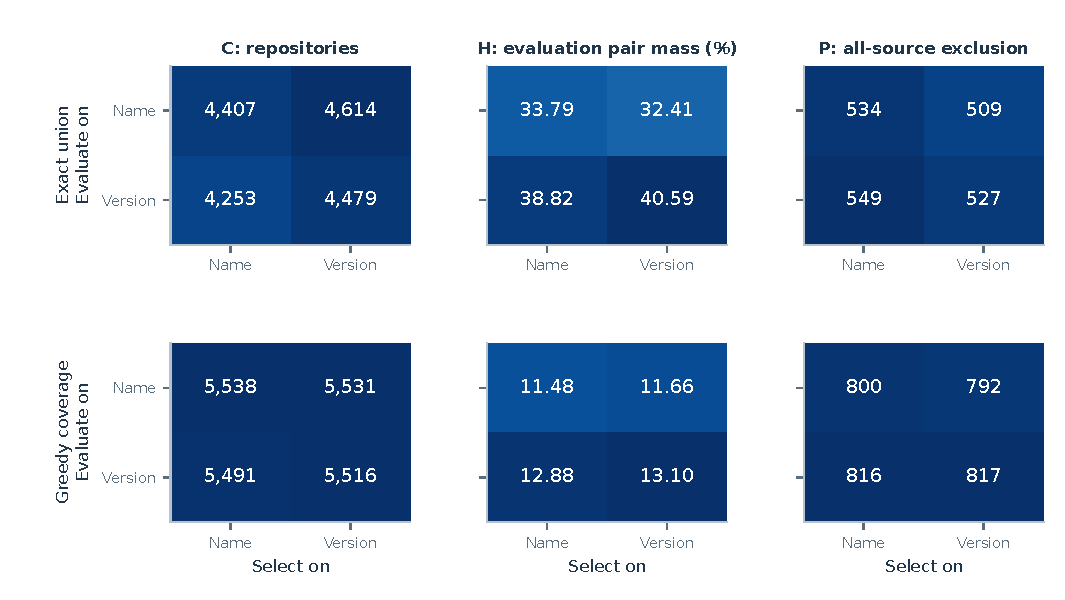
\includegraphics[width=0.98\textwidth]{representation_matrix.pdf}
\caption{Budget-100 selection/evaluation combinations for exact union and greedy. C and P count workflow repositories; H is divided by all account--repository pairs in the evaluation representation (462,170 for names; 266,016 for versions). Panels are separate metrics, not a common color scale.}
\label{fig:q1_representation_matrix}
\end{figure*}

Figure~\ref{fig:q1_representation_matrix} separates the representation used for selection from the one used for evaluation. Comparisons of H within an evaluation row share a denominator; comparisons across rows change that denominator. A change in representation can therefore change both the selection and the quantity being measured.

\section{Exclusion Heuristic Validation: RQ3}
\label{sec:pareto_and_weights}
\subsection{Baseline Gain and Component Ablations}
On the original graph, the direct heuristic yields $P=1{,}022$ at budget 100, compared with greedy coverage's 800 and exact union's 534. This gain comes with $C=5{,}020$ and $H=13.23\%$; it does not maximize every objective. Table~\ref{tab:q1_supermodular_p} retains the multi-budget comparison.
% Auto-generated Supermodular P(S) Optimization Table for Q1 Journal Expansion
\begin{table*}[t]
\centering
\small
\caption{All-source exclusion $P(S)$ optimization via greedy minimum-source heuristic versus baseline single-objective rankings.}
\label{tab:q1_supermodular_p}
\begin{tabular}{rrrrrrrr}
\toprule
Budget & \multicolumn{3}{c}{Direct $P(S)$ Heuristic} & Greedy $P$ & Union $P$ & Gain vs Gr. & Gain vs Un.\\
\cmidrule(lr){2-4}
$|S|$ & $P$ & $C$ (\%) & $H$ (\%) & & & $\Delta P$ & $\Delta P$\\
\midrule
10 & \textbf{479} & 55.4\% & 2.58\% & 351 & 343 & +128 & +136\\
25 & \textbf{618} & 59.1\% & 4.15\% & 514 & 427 & +104 & +191\\
50 & \textbf{803} & 64.2\% & 6.55\% & 638 & 441 & +165 & +362\\
100 & \textbf{1,022} & 70.0\% & 13.23\% & 800 & 534 & +222 & +488\\
\bottomrule
\end{tabular}
\end{table*}


\begin{figure}[t]
\centering
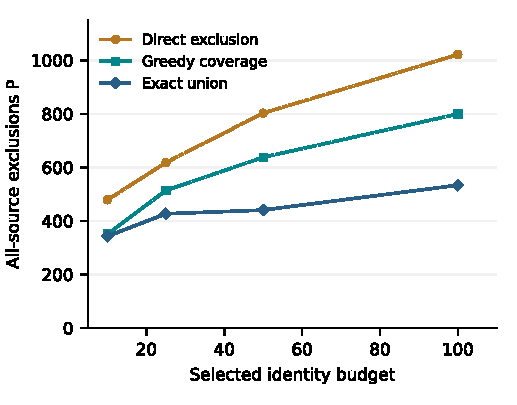
\includegraphics[width=\columnwidth]{q1_supermodular_p.pdf}
\caption{All-source exclusion under the original heuristic and coverage/exposure baselines. Counts describe the retained graph under ideal selected-source hardening.}
\label{fig:q1_supermodular_p_weights}
\end{figure}

The new runner parameterizes the original lexicographic rule and reproduces its complete retained 100-account order before introducing variants. It changes the candidate cap to 1, 5, 20 and unrestricted, removes reciprocal remaining-source scoring or the coverage tie-break, and repeats tied choices under 30 frozen seeds. These are component sensitivities, not independent ecosystem observations.
% Generated by scripts/render_journal_validation.py
\begin{table*}[t]
\centering
\footnotesize
\caption{Budget-100 component ablations on the original graph. Timing is one selection run in the same process.}
\label{tab:revision_heuristic}
\begin{tabular}{lrrrr}
\toprule
Rule & $C$ & $H$ (\%) & $P$ & Seconds\\
\midrule
Original rule (cap 10) & 5,020 & 13.23 & 1,022 & 19.56\\
Immediate + coverage & 5,043 & 11.75 & 1,024 & 13.65\\
No coverage tie-break & 5,020 & 13.23 & 1,022 & 13.64\\
Cap 1 & 5,020 & 13.23 & 1,022 & 4.96\\
Cap 5 & 5,020 & 13.23 & 1,022 & 11.45\\
Cap 20 & 5,020 & 13.23 & 1,022 & 17.63\\
No candidate cap & 5,020 & 13.23 & 1,022 & 89.10\\
\bottomrule
\end{tabular}
\par\smallskip\begin{minipage}{0.98\textwidth}\footnotesize Immediate + coverage omits reciprocal remaining-source scoring and is identical to the no-reciprocal variant. Thirty seeded tie runs each give $P=1{,}022$ at budget 100; this is selection variability on one graph, not ecosystem uncertainty.\end{minipage}
\end{table*}


Removing reciprocal scoring gives $P=1{,}024$, two more than the original rule, together with $C=5{,}043$ and $H=11.75\%$. The immediate-completion variant uses coverage then identity order to resolve zero-gain cases. Candidate-cap changes and removing the coverage tie-break retain the original budget-100 P on this graph. All 30 tie runs also yield $P=1{,}022$. These outcomes provide no evidence that the reciprocal term improves original-graph exclusion; its usefulness must be assessed across other observed populations. Single-run timing in Table~\ref{tab:revision_heuristic} characterizes the implementation rather than a hardware-independent performance guarantee.

\subsection{Candidate-Restricted Exact Benchmarks}
We freeze 20 empirical candidate pools and 12 synthetic overlap instances, each with 20 eligible accounts and budgets 1, 3 and 5. Exhaustive enumeration evaluates every eligible subset. Empirical instances preserve complete endpoint source sets: sources outside the candidate pool remain unselected and can prevent exclusion. Candidate pools are constructed from low-cardinality source sets and reach-ranked fill accounts, so these are tractable diagnostic instances rather than a random sample of full-graph optimization problems.
% Generated by scripts/render_journal_validation.py
\begin{table*}[t]
\centering
\footnotesize
\caption{Exact exclusion benchmarks with 20 eligible accounts and budgets 1, 3 and 5.}
\label{tab:revision_exact}
\begin{tabular}{lrrrr}
\toprule
Instance family & Settings & Exact hits & Worst gap & Min ratio (\%)\\
\midrule
Empirical candidate pools & 60 & 51 & 66 & 16.46\\
Synthetic overlap instances & 36 & 35 & 1 & 93.33\\
\bottomrule
\end{tabular}
\par\smallskip\begin{minipage}{0.98\textwidth}\footnotesize Twenty empirical pools and twelve synthetic instances each supply three correlated budget settings. Outside-candidate sources remain unselected. Optima apply only to the restricted instance; no full-graph approximation guarantee follows.\end{minipage}
\end{table*}


The original heuristic reaches the restricted optimum in \HeuristicExactHits{} of \HeuristicExactSettings{} settings. It matches 51 of 60 empirical settings and 35 of 36 synthetic settings. Its worst empirical deficit is \HeuristicWorstGap{} endpoints and its minimum achieved-to-optimal ratio is 16.46\%; the worst synthetic deficit is one endpoint. Figure~\ref{fig:revision_audit_benchmarks}(b) shows the gap distributions. The 96 settings reuse 32 instances across budgets and are not independent replicates. These diagnostics identify substantive failure cases; neither the hit count nor the synthetic results certify the original full graph's optimum or an approximation ratio.

\subsection{Other Objective Choices}
Standard scalarization exposes intermediate coverage--exposure choices, but a preferred weight requires review costs and stakeholder preferences that were not measured. Additional heterogeneous weights, strict thresholds and uniform-efficacy multipliers are reported in Appendix~\ref{sec:objective_supplement}. A threshold sensitivity is not a count of empirically protected repositories: source identities are not authenticated approval groups, and the study does not observe an enforced release policy.

\section{Historical Metadata and Acquisition Feasibility}
\label{sec:temporal_authority}
The historical companion asks what retained registry metadata can support before an event cutoff. It is separate from the cross-sectional reverse-reach experiment. It does not test whether the primary rankings would have predicted historical compromise.

\subsection{Bounded Cutoff-SemVer Reconstruction}
For each retained root record, the reconstruction chooses the highest currently retained, non-prerelease version satisfying a runtime dependency range and published by the root cutoff. Expansion stops at depth three or 250 nodes per root. Peer, optional, development, bundled, workspace, override, git, and tarball dependency behavior is excluded. Deleted historical versions may be unavailable; present-day retention cannot recreate every past registry state.

Table~\ref{tab:q1_temporal_reconstruction} summarizes the bounded reconstruction.
% Generated by scripts/reconcile_full_manuscript.py
\begin{table*}[t]
\centering
\footnotesize
\caption{Retained bounded registry-SemVer reconstruction manifest. The recorded resolution share is conditional on attempted expansions within the bounds.}
\label{tab:q1_temporal_reconstruction}
\begin{tabular}{lr}
\toprule
Recorded dimension & Value\\
\midrule
Retained root records & 45\\
Distinct event/root/cutoff tuples & 44\\
Recorded edge attempts & 1,848\\
Resolved recorded edges & 1,841\\
Node counts summed over roots & 1,272\\
Unresolved expansions & 7\\
Resolved share of recorded attempts & 99.62\%\\
Maximum expansion depth & 3\\
Node cap per root & 250\\
Roots reaching cap & 1\\
\bottomrule
\end{tabular}
\par\smallskip\begin{minipage}{0.98\textwidth}\footnotesize Only regular dependencies are included; depth is capped at three and nodes at 250 per root. Highest retained cutoff-valid satisfying versions are used. These are bounded approximations, not lockfile reconstructions or completeness guarantees. Raw-response checksums establish retained-object identity, not publisher authenticity.\end{minipage}
\end{table*}


The source contains 45 root records but 44 distinct event/root/cutoff tuples: one \texttt{node-ipc} tuple is repeated. We report retained-record counts without treating them as independent incidents. Of 1,848 recorded edge attempts, 1,841 resolve and seven have unavailable target registries, yielding 99.62\% among recorded attempts. This percentage excludes unvisited expansions beyond the bounds. The 1,272 node count is summed across roots, not globally deduplicated. One record reaches the node cap. These measurements do not establish full-tree completeness, downstream population reconstruction, or unbiased historical rankings.

\subsection{Release-Field Availability and Authority Limits}
Table~\ref{tab:q1_release_authority} reports the availability of release fields.
% Generated by scripts/reconcile_full_manuscript.py
\begin{table*}[t]
\centering
\footnotesize
\caption{Field availability in 45 retained pre-event version-object records. Comparison availability is not continuity, equality, or authenticated release authority.}
\label{tab:q1_release_authority}
\begin{tabular}{lrr}
\toprule
Metadata availability & Count & Share\\
\midrule
Retained selected-version objects & 45 & 100.0\%\\
Immediate predecessor available & 44 & 97.8\%\\
Repository-field comparison available & 42 & 93.3\%\\
gitHead-field comparison available & 34 & 75.6\%\\
publishConfig comparison available & 11 & 24.4\%\\
Selected dist.integrity present & 45 & 100.0\%\\
Selected embedded maintainers present & 45 & 100.0\%\\
\bottomrule
\end{tabular}
\par\smallskip\begin{minipage}{0.98\textwidth}\footnotesize The 45 records include a repeated event/root/cutoff tuple; they are not independent incidents. Embedded maintainer metadata is not a signature. No version-specific provenance endpoint requests, bundle retrievals, signature verifications, or attestation-state classifications were performed. Historical attestation presence/absence is unknown, not 0/45 absent.\end{minipage}
\end{table*}


The availability audit finds predecessor metadata for 44 of 45 retained records, repository-field comparison availability for 42, and \texttt{gitHead}-field comparison availability for 34. Availability does not show that URLs stayed equal, commits were valid or available, or a publisher retained authority. The audit classified no field deltas, built no authority scores, and evaluated no release-gating control.

All 45 records contain \texttt{dist.integrity} and embedded maintainer metadata. A distribution hash identifies expected artifact bytes; an embedded maintainer array is not a cryptographic signature. Neither proves a benign or reproducible build. The attestation access assessment made no version-specific requests, retrieved no bundles, ran no signature verification, and classified no attestation states. Historical attestation presence is therefore \emph{unknown}; zero retrievals cannot be reported as zero attestations. Signing studies motivate the need for stronger evidence~\cite{okafor2025,schorlemmer2024}, without supplying the missing measurements for this cohort.

The LiteLLM source-tag/artifact discrepancy~\cite{litellmincident2026} illustrates why artifact identity, intended source, and release authority must be evaluated separately. Contextual reports do not add observations to the 45-record companion.

\subsection{Metadata-Acquisition Pilot}
A separate metadata pilot sampled 100 identifiers uniformly without replacement from the original 25,228-identifier frame (seed 20261020). Of 92 ordinary-shaped names, 90 yielded metadata and two returned HTTP 404; all eight bundled-context identifiers returned HTTP 405. No identifier was replaced. The acquisition cutoff was October 20, 2026, 00:48:38 Asia/Dhaka. The pilot characterizes retrieval feasibility and sampling-frame defects; it includes no measured incident outcomes or forecasting evaluation.

\section{Threats to Validity and Research Ethics}
\label{sec:threats_to_validity}
We organize limitations around construct, internal, external, and conclusion validity, informed by empirical reporting guidance~\cite{ralph2020}.

\subsection{Construct Validity}
Registry maintainer arrays supply username associations, not historical publication authority, token scope, account independence, or a peer-review policy. One maintainer does not prove absence of human review; several do not prove enforced review. Uniform and heterogeneous source weights are modeling assumptions. The perfect hardening model removes selected account origins, not package nodes or paths from other origins.

The workflow observation is a directory lookup at HEAD. We did not retain workflow YAML, job execution, permission scopes, historical release links, or consumer lockfiles. Dependency and workflow association therefore establishes neither installation nor vulnerable-code execution or secret access. CI dependency studies~\cite{weeraddana2024} and finer-grained vulnerability analysis~\cite{gao2025emse} motivate those distinctions without supplying execution evidence for our endpoints.

The main exact-version graph is an observed deps.dev edge union, while the temporal companion is a bounded highest-satisfying SemVer approximation. They are different representations. Neither reconstructs npm hoisting, installed versions, overrides, or complete historical dependency trees. Runtime vulnerabilities such as the Node.js Brotli disclosure~\cite{nodejsbrotli2026} are outside the package graph. Residual thresholds are hypothetical source-count rules, without signer groups, role constraints, or measured enforcement.

\subsection{Internal and Observational Validity}
Independent traversals, transposed source incidence, small-graph cases, and generated result checks validate computations on retained evidence. They cannot recover omitted observations. SCC condensation preserves reach; it is not a source of measured cycle-removal benefit. Ties use ascending username order, not portfolio size, except where portfolio size defines the selection rule itself.

Repository normalization is lexical. Excluding inconsistent positive observations tests sensitivity; it does not validate the other remote mappings or repair historical flags. Both main representations mix contexts and acquisition dates. Unknown workflow states and ambiguous zeros can omit eligible endpoints. Historical availability counts describe retained records, including a repeated tuple, and do not establish independent incidents or verified release authority.

\subsection{External and Conclusion Validity}
The high-impact-seeded expansion is neither registry-wide nor a random sample of npm installations. Public workflow-associated repositories cannot represent private consumer infrastructure without further evidence. Results describe this graph and explicit scenarios. They supply no measured compromise probabilities or causal control effects.

Random orders quantify selection variability. Orders are reused across nested budgets and endpoint definitions, so the resulting 6,000 rows are not independent ecosystem samples. Monte Carlo errors describe simulation means, not npm-wide uncertainty. The seven scalarization settings are exploratory tradeoff points, without a certified global Pareto frontier or an empirically estimated stakeholder preference. Heterogeneous weights are structural sensitivities, not fitted risk priors. Claims about efficacy require a separate intervention study.

\subsection{Ethics and Reporting}
The analyses read retained public metadata and execute no package payloads, credential probes, or exploitation. Prospective captures omit email addresses and package bodies. Public usernames illustrate structural overlap without implying present-day insecurity, negligence, or historical publishing authority. Incident associations do not validate prediction. Artifact checksums identify retained bytes rather than certify authenticity. Assistance is disclosed, and authors must review the claims, sources, code, and applicable submission requirements.

\section{Conclusion}
\label{sec:conclusion}
Maintainer selection depends on the quantity a review program seeks to improve. In the original graph, budget-100 greedy covers 5,538 repositories and exact union 4,407, with uniform-scenario exposure reductions of 11.48\% and 33.79\%. The direct exclusion heuristic increases P from greedy's 800 to 1,022, but omitting reciprocal scoring yields 1,024. Candidate-cap and tie sensitivities leave the original heuristic's final P unchanged, while restricted exact instances reveal deficits as large as 66 endpoints.

A fresh 100-root acquisition supplies 66 workflow-associated repository endpoints and repeats the coverage--exposure tradeoff. Greedy reaches 65 and exact union 42, while the direct heuristic excludes all sources for 34 endpoints. Version continuity decreases pair mass by 3.33\% in this cohort, compared with 42.44\% in the original union. The shared direction and differing magnitude support explicit population, representation and denominator choices rather than a universal numeric correction or preferred account list.

The frozen 120-endpoint audit acquires 115 pinned commits and prepares independent author review. Its machine labels remain provisional and establish neither executed dependencies nor validated historical mapping precision. Historical metadata reconstruction and prospective outcome feasibility remain appendices with no forecasting result. The completed computations support structural prioritization comparisons and documented failure cases; evaluating actual control effectiveness requires additional authority, installation and intervention evidence.


\section*{Acknowledgment}
The authors thank npm package maintainers and the open-source community for making studied artifacts publicly available, and deps.dev and GitHub for data interfaces. Per venue policy, a large language model was employed solely for non-intellectual grammatical polishing and typesetting assistance; all study design, implementations, analyses, and scientific conclusions were conducted and verified by the authors.

\bibliographystyle{IEEEtran}
\bibliography{bibliography/references_q1}

\end{document}
